\section{Practical Aspects}

We address here some issues that arise when implementing the described algorithm on a resource-constrained platform. Furthermore, we introduce many practical expedients that deal with limited sampling budget, slow control rates and finally with sim-to-real transfer.  

\subsection{Gradient Clipping} 
The policy update rule in \eqn \ref{eq:update_rule} consists of a receding horizon \emph{mini-batch} SGD. As a consequence, the gradient variance can vary greatly between successive iterations of the algorithm. To prevent this phenomenon, which is especially evident with a small sampling budget, we clip the gradients to a user-defined threshold.  

\subsection{Receding Horizon Control} 
Model-based predictive control rarely achieves the rate of common low-level controllers because of the time consuming rollouts sampling. Nevertheless, the generated input sequence can be used in open loop by a cascaded joint velocity trajectory tracking controller. 

At the beginning of a new sampling, all the stored rollouts are shifted back by the real-time number of steps elapsed since the last optimization. A subset of the best rollouts are kept to warm start the next iteration. 
As the sampled control is not sufficiently smooth for a practical application, we filter if using a moving window Savitzky-Golay filter~\cite{gorry1990general} before the FILTER-QP. 

\subsection{Adaptive temperature} 
The coefficient $\lambda$ in \eqref{eq:weighting} determines how much ``aggressive" the weighting between different trajectories is. Adopting a constant value would give a numerically zero weight to most of the trajectories. Shifting the trajectory cost by the minimum cost as proposed in~\cite{williams_information_2017} also does not alleviate this issue. 
Especially in regions of high cost, trajectories that are equivalently good can be assigned very different weights. We instead propose to adopt the same technique as in~\cite{theodorou2010generalized} where the parameter $\lambda$ can be automatically optimized to maximally discriminate between the experienced trajectories. The modified exponential utility is then defined by,
\begin{equation} \label{eq:adaptive_t}
    \exp (-\lambda J ) = \exp \left( -h \frac{J - J_{\min}}{J_{\max} - J_{\min}} \right).
\end{equation}

\subsection{Chattering}
We observed that a naive implementation of the passivity constraint leads to a chattering behavior at the constraint boundary. We start discretizing the constraint inequality to obtain a constraint which is affine in the input $\command$:
\begin{equation*}
    \int_{0}^{\sigma} \boldsymbol{\tau}_{ext}^T \command \ dt \approx \underbrace{\boldsymbol{\tau}_{ext}(t + dt)^T \command(t+dt) dt}_{P_{diss}} + S(x_t(t)) \geq \epsilon
\end{equation*}
which is equivalent to 
\begin{equation}
    P_{diss} \leq \alpha E_{res}
\end{equation}

where we defined the residual energy $S(x_t(t))-\epsilon$ as $E_{res}$. The above inequality has the drawback that when the Euler integration is performed with small time intervals, then a dangerously high power can be dissipated at any time, until very close to the lower energy limit, thus leading to chattering. It is therefore better to use a value of $\alpha > 1/dt$. One can easily verify that defining a passivity ZBF as $h_{pass} = S(x_t) - \epsilon$ we obtain the same formulation. The ZBF constraint reads as: 
\begin{align}
    \dot{h}_{pass} &= \dot{S}(x_t) \\
     &\geq -\alpha h_{pass} \\
     &=\alpha (\epsilon - S(x_t)))
\end{align}
The passivity can therefore seen as a ZBF and consequently inherits its properties. A smaller value for $\alpha$ can be seen as making the constraint more conservative and improve its performance an the boundary. This effect is show in \fig \ref{fig:tank_as_zbf} in the experiment section.

\subsection{Simulator tuning}
Crucial to the overall performance is the accuracy of the simulation environment (implementing \eqn \ref{eq:eom}). Unfortunately the discrepancy between the simulator and the real physical model known as the \emph{sim-to-real} gap is always present. A typical failure case consists of an over-estimation of an object's friction. In such cases, we have often observed a ``scratching" emergent behavior where the robot would rely on friction to move the object. In practice friction is hard to measure and depends on the contact patch between surfaces. On the other hand, kinematic constraints between contact points depends on the system geometry which can be accurately measured (e.g from CAD models). Therefore solutions that exploit the latter are more likely to succeed on the real platform. One can bias the controller towards these solutions by setting, for example, a very low friction coefficient between contact bodies.

\subsection{Contact-mesh simplification}
A large proportion of simulation time is spent on collision detection. We reduce the component meshes to the relevant ones and simplify to primitive shapes, as shown in \fig\ref{fig:1}. We are especially interested in the collision objects belonging to the robot end-effector and the object. This adaptation tremendously reduces computation especially during the contact phase. In our following evaluations we observed that using the original mesh shown in \fig\ref{fig:original_mesh} results in a mean simulation rate of 0.98kHz. In contrast, the two finger mesh and hook finger mesh in \fig\ref{fig:two_fingers}-\ref{fig:hook_finger} allow mean simulation rates of 2.13kHz and 2.94kHz, respectively.

\begin{figure}[t]
\centering
\begin{subfigure}{0.3\columnwidth}
    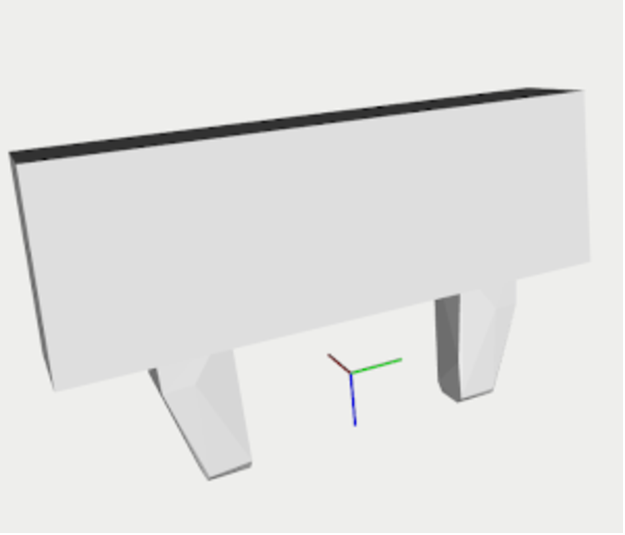
\includegraphics[width=\linewidth]{framework_manipulation/figures/hardware/mesh_cropped.pdf}
    \caption{Original mesh}\label{fig:original_mesh}
\end{subfigure}%
\hfill
\begin{subfigure}{0.3\columnwidth}
    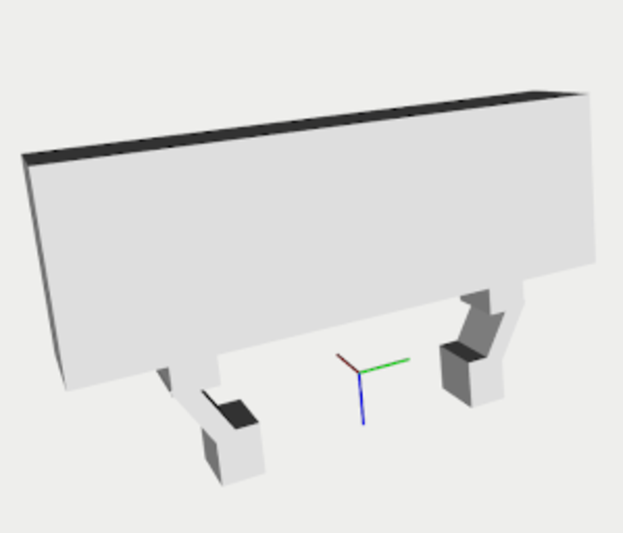
\includegraphics[width=\linewidth]{framework_manipulation/figures/hardware/doulbe_simple_cropped.pdf}
    \caption{Two fingers}\label{fig:two_fingers}
\end{subfigure}%
\hfill
\begin{subfigure}{0.3\columnwidth}
    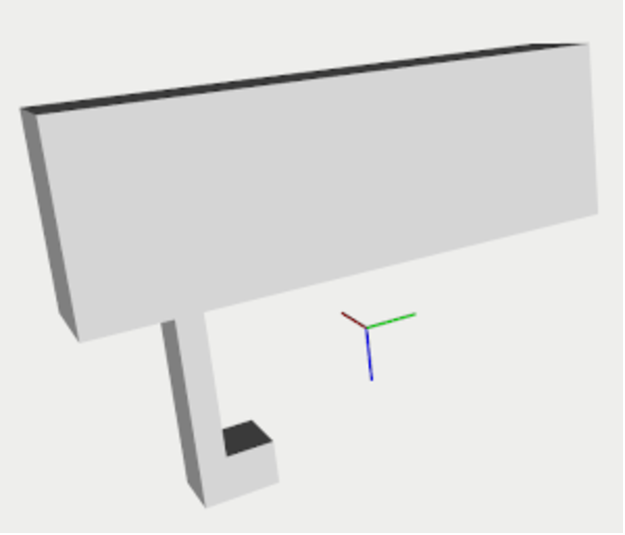
\includegraphics[width=\linewidth]{framework_manipulation/figures/hardware/single_hook_cropped.pdf}
    \caption{Hook finger}\label{fig:hook_finger}
\end{subfigure}
% \subfloat{%
%     \begin{tabular}{c|c|c|c}
%              &  (a) & (b) & (c) \\ 
%                       \hline
%          Mean sim rate & 0.98 KHz & 2.13 KHz & 2.94 KHz\\
%     \end{tabular}
%     \label{subtbl:the-table}
%   }

\caption{Original collision meshes are often approximated by convex hulls which are inaccurate while also more complex representations. In contrast, a simplified mesh can bring more accuracy as well as a computational performance gain in terms of simulation rate.}\label{fig:1}

\end{figure}

 
\subsection{Cascaded control architecture}
The expensive rollout sampling procedure often limits the rate of the controller. Instead, the QP can be efficiently solved at almost the same rate as the low-level controller. We propose a \emph{cascaded control} architecture composed of a low-rate policy update block and a high-rate low-level control loop. The latter solves the FILTER-QP in \eqn \eqref{eq:cbf-qp} point-wise to find the best input according to the latest received measurements. 
\begin{figure}[t!]
\centering
\hspace*{-0.7cm}
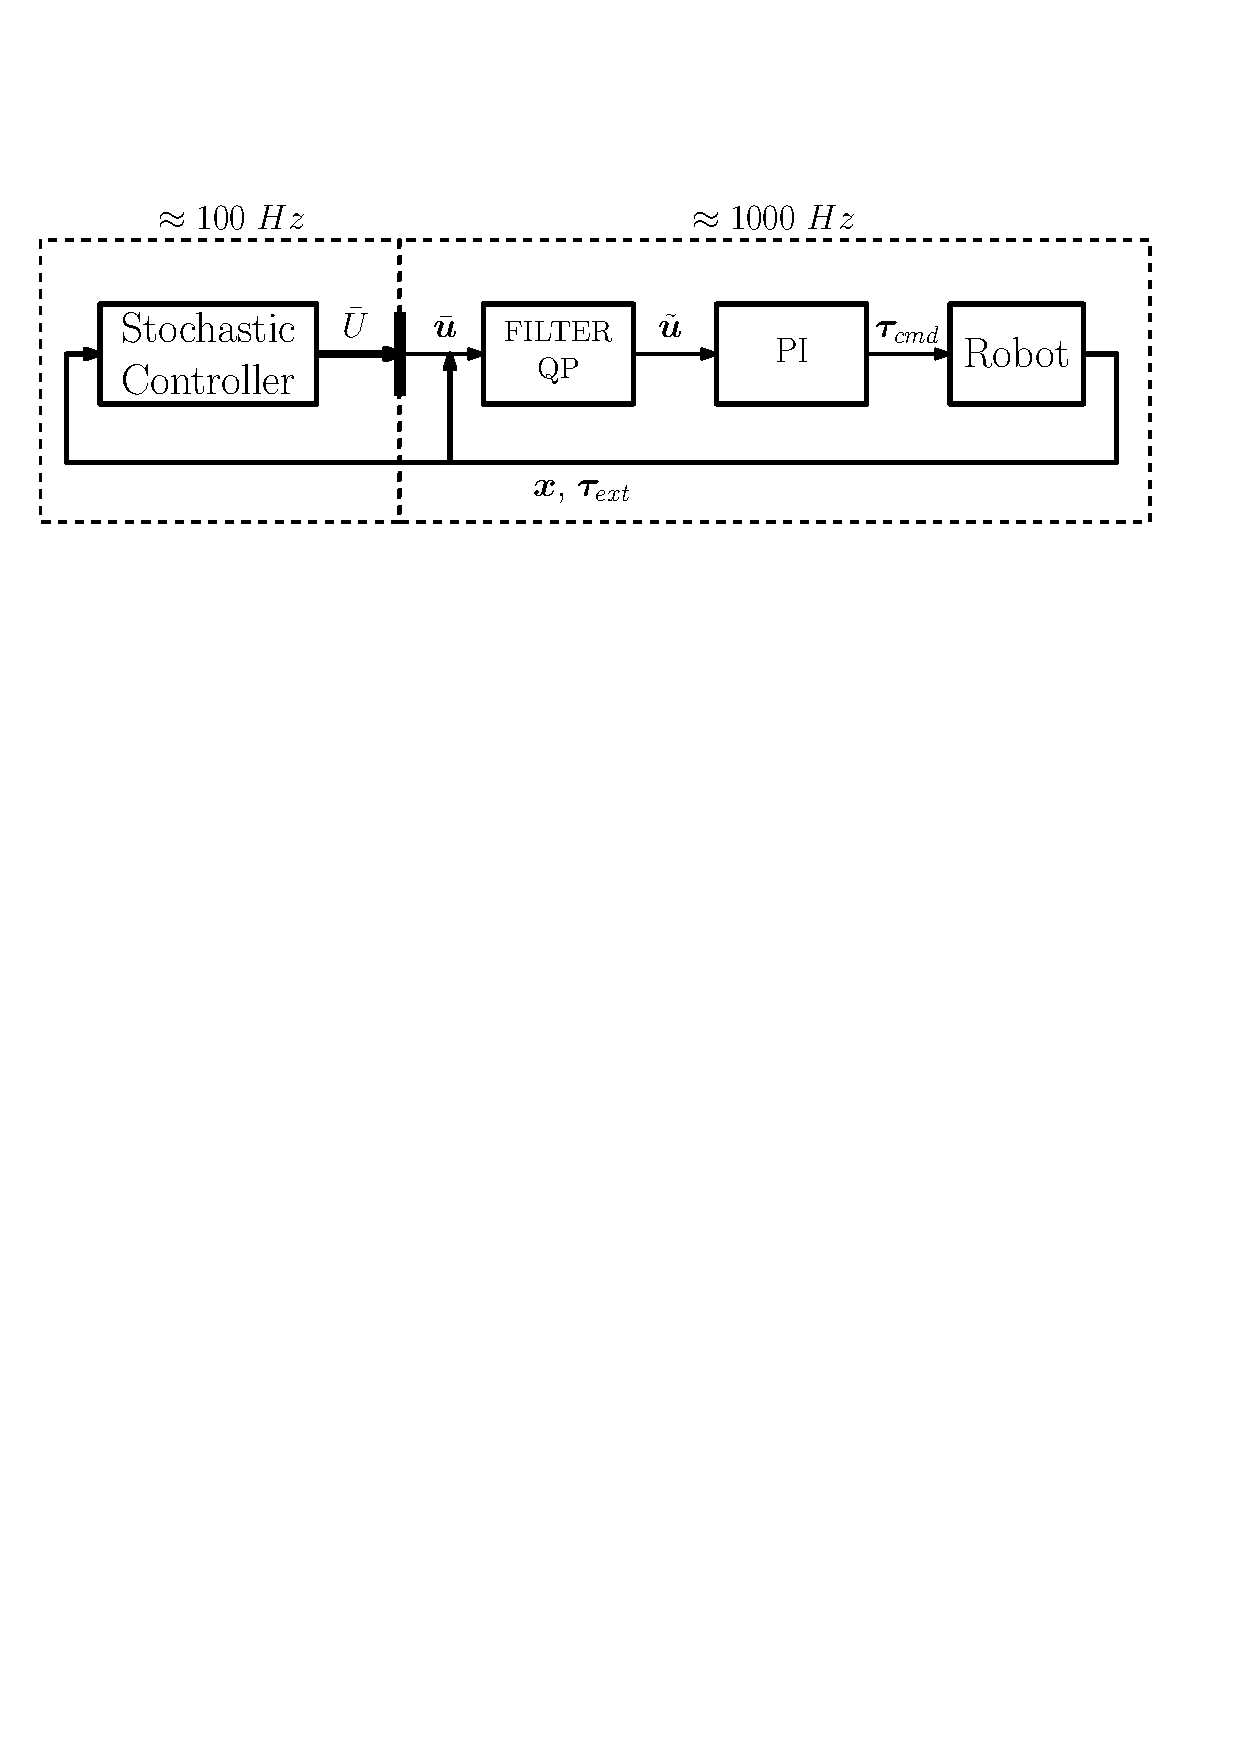
\includegraphics[width=1.1\columnwidth]{figures/schemes/high_level_architecture.pdf}
\caption{Cascaded control architecture: the stochastic controller computes a velocity trajectory $\bar{U}$ at approximately 100Hz. The input vector is queried and interpolated at a higher rate of approximately 1000Hz (tick line) and is filtered using the latest odometry.} \label{fig:cascaded_architecture}
\end{figure}

